
%Dokumentinformationen
\newcommand{\titleinfo}{Analysis 2E - Formelsammlung}


\newcommand{\authorinfo}{F. Braun, L. Schmid, U. Giger, R. Koller, E. Ammann, S. Arnold, C. Gwerder, S. Koerner, L. Leuenberger}
\newcommand{\versioninfo}{$Revision: $ \today}


% standard header
%Schriftgr�sse, Layout, Papierformat, Art des Dokumentes
\documentclass[10pt,twoside,a4paper,fleqn]{article}
%Einstellungen der Seitenr�nder
\usepackage[left=1cm,right=1cm,top=1cm,bottom=1cm,includeheadfoot]{geometry}
% Sprache, Zeichensatz, packages
\usepackage[utf8]{inputenc}
\usepackage[ngerman]{babel,varioref}
\usepackage{amssymb,amsmath,fancybox,graphicx,color,lastpage,wrapfig,fancyhdr,hyperref,verbatim}

%pdf info
\hypersetup{pdfauthor={\authorinfo},pdftitle={\titleinfo},colorlinks=false}
%linkbordercolor=white
\author{\authorinfo}
\title{\titleinfo}

%Kopf- und Fusszeile
\pagestyle{fancy}
\fancyhf{}
%Linien oben und unten
\renewcommand{\headrulewidth}{0.5pt} 
\renewcommand{\footrulewidth}{0.5pt}

\fancyhead[L]{\titleinfo{ }\tiny{(\versioninfo)}}
%Kopfzeile rechts bzw. aussen
\fancyhead[R]{Seite \thepage { }von \pageref{LastPage}}
%Fusszeile links bzw. innen
\fancyfoot[L]{\footnotesize{\authorinfo}}
%Fusszeile rechts bzw. ausen
\fancyfoot[R]{\footnotesize{\today}} % ./header.tex nicht editieren (Projekt LaTeX-Header benutzen)


% This is needed for one more subsection, ex. 1.1.1.1, is called by \paragraph{}
\usepackage{titlesec}
\setcounter{secnumdepth}{4}
\setcounter{tocdepth}{4}
\titleformat{\paragraph}
{\normalfont\normalsize\bfseries}{\theparagraph}{1em}{}
\titlespacing*{\paragraph}
{0pt}{2.25ex plus 1ex minus .2ex}{1.0ex plus .2ex}

% This is needed for a smaller itemlist, is called by \compactenum {}
\usepackage{paralist}

% This is needed for merging some columns in a table
\usepackage{multicol} 
\usepackage{multirow} 

\begin{document}
\setlength{\parindent}{0pt}
           
%%%%%%%%%%%%%%%%%%%%%%%%%%%%%%%%%%%%%%%%%%%%%%%%%%%%%%%%%%%%%%%%%%%%%%%%%%%%%%%%%%%%%%%%%%%%%%%%
%%%%%%%%%%%%%%%%%%%%%%%%%%%%%%%%%%%%%%%%%%%%%%%%%%%%%%%%%%%%%%%%%%%%%%%%%%%%%%%%%%%%%%%%%%%%%%%%

\section{Integralrechnung \formelbuch{492}}
\subsection{Integrationsmethoden \formelbuch{495ff}}

\renewcommand{\arraystretch}{2}
\begin{tabular}{| l | l |}
	\hline
		Linearität &
			$\int{f(\alpha x+\beta )dx=\frac{1}{\alpha}\cdot F(\alpha x+\beta)+C}$ \\
	\hline
		Partielle Integration &
			$\int\limits_a^b{u'(x)\cdot v(x)dx}=\biggl[ u(x)\cdot v(x) \biggr]_a^b-\int\limits_a^b{u(x)\cdot v'(x)dx}$ \\
	\hline
		Weierstrass-Substitution &
			$t=\tan\frac{x}{2}, \qquad dx=\frac{2dt}{1+t^2}$
			$\qquad \sin  x=\frac{2t}{1+t^2}$
			$\qquad \cos x=\frac{1-t^2}{1+t^2} \quad\int{R(\sin(x),\cos(x))dx}$ \\
	\hline
		Allgemeine Substitution &
			$\int\limits_{a}^{b}{f(x)dx}=\int\limits_{g^{-1}(a)}^{g^{-1}(b)}{f(g(t))\cdot g'(t)dt}$
			$\qquad t=g^{-1}(x)$
			$\qquad  \fbox{x=g(t)}\Leftrightarrow^{d(...)} dx=g'(t)\cdot dt$ \\
	\hline
		Logarithmische Integration &
			$\int{\frac{f'(x)}{f(x)}dx}=\ln|f(x)|+C$
			$\qquad {(f(x)\neq 1)}$
			$\qquad y'(x)\cdot dx = dy \rightarrow$ allg. gültig\\
	\hline
		Potenzregel &
			$\int{f'(x)\cdot (f(x))^{\alpha} dx}=\frac{f(x)^{\alpha +1}}{\alpha+1}+C$
			$\qquad{(\alpha \neq -1)}$ \\
	\hline
		Differentiation &
			$\int \limits ^{b} _{a} {f'(t)dt}=f(b)-f(a)$
			$\qquad \frac{d}{dx} \int \limits ^{x} _{1} {f(t)dt}=f(x)$ \\
	\hline
			Mittelwerte &
				linear: $\frac{1}{b-a} \int\limits ^{b} _{a} {f(x)dx}$
				$\qquad$ quadratisch: $\sqrt{\frac{1}{b-a} \int\limits ^{b} _{a} {\lvert f(x)^2 \rvert dx}}$ \\
	\hline
\end{tabular}
\renewcommand{\arraystretch}{1}


\subsubsection{Einige unbestimmte Integrale \formelbuch{1081ff}} 
 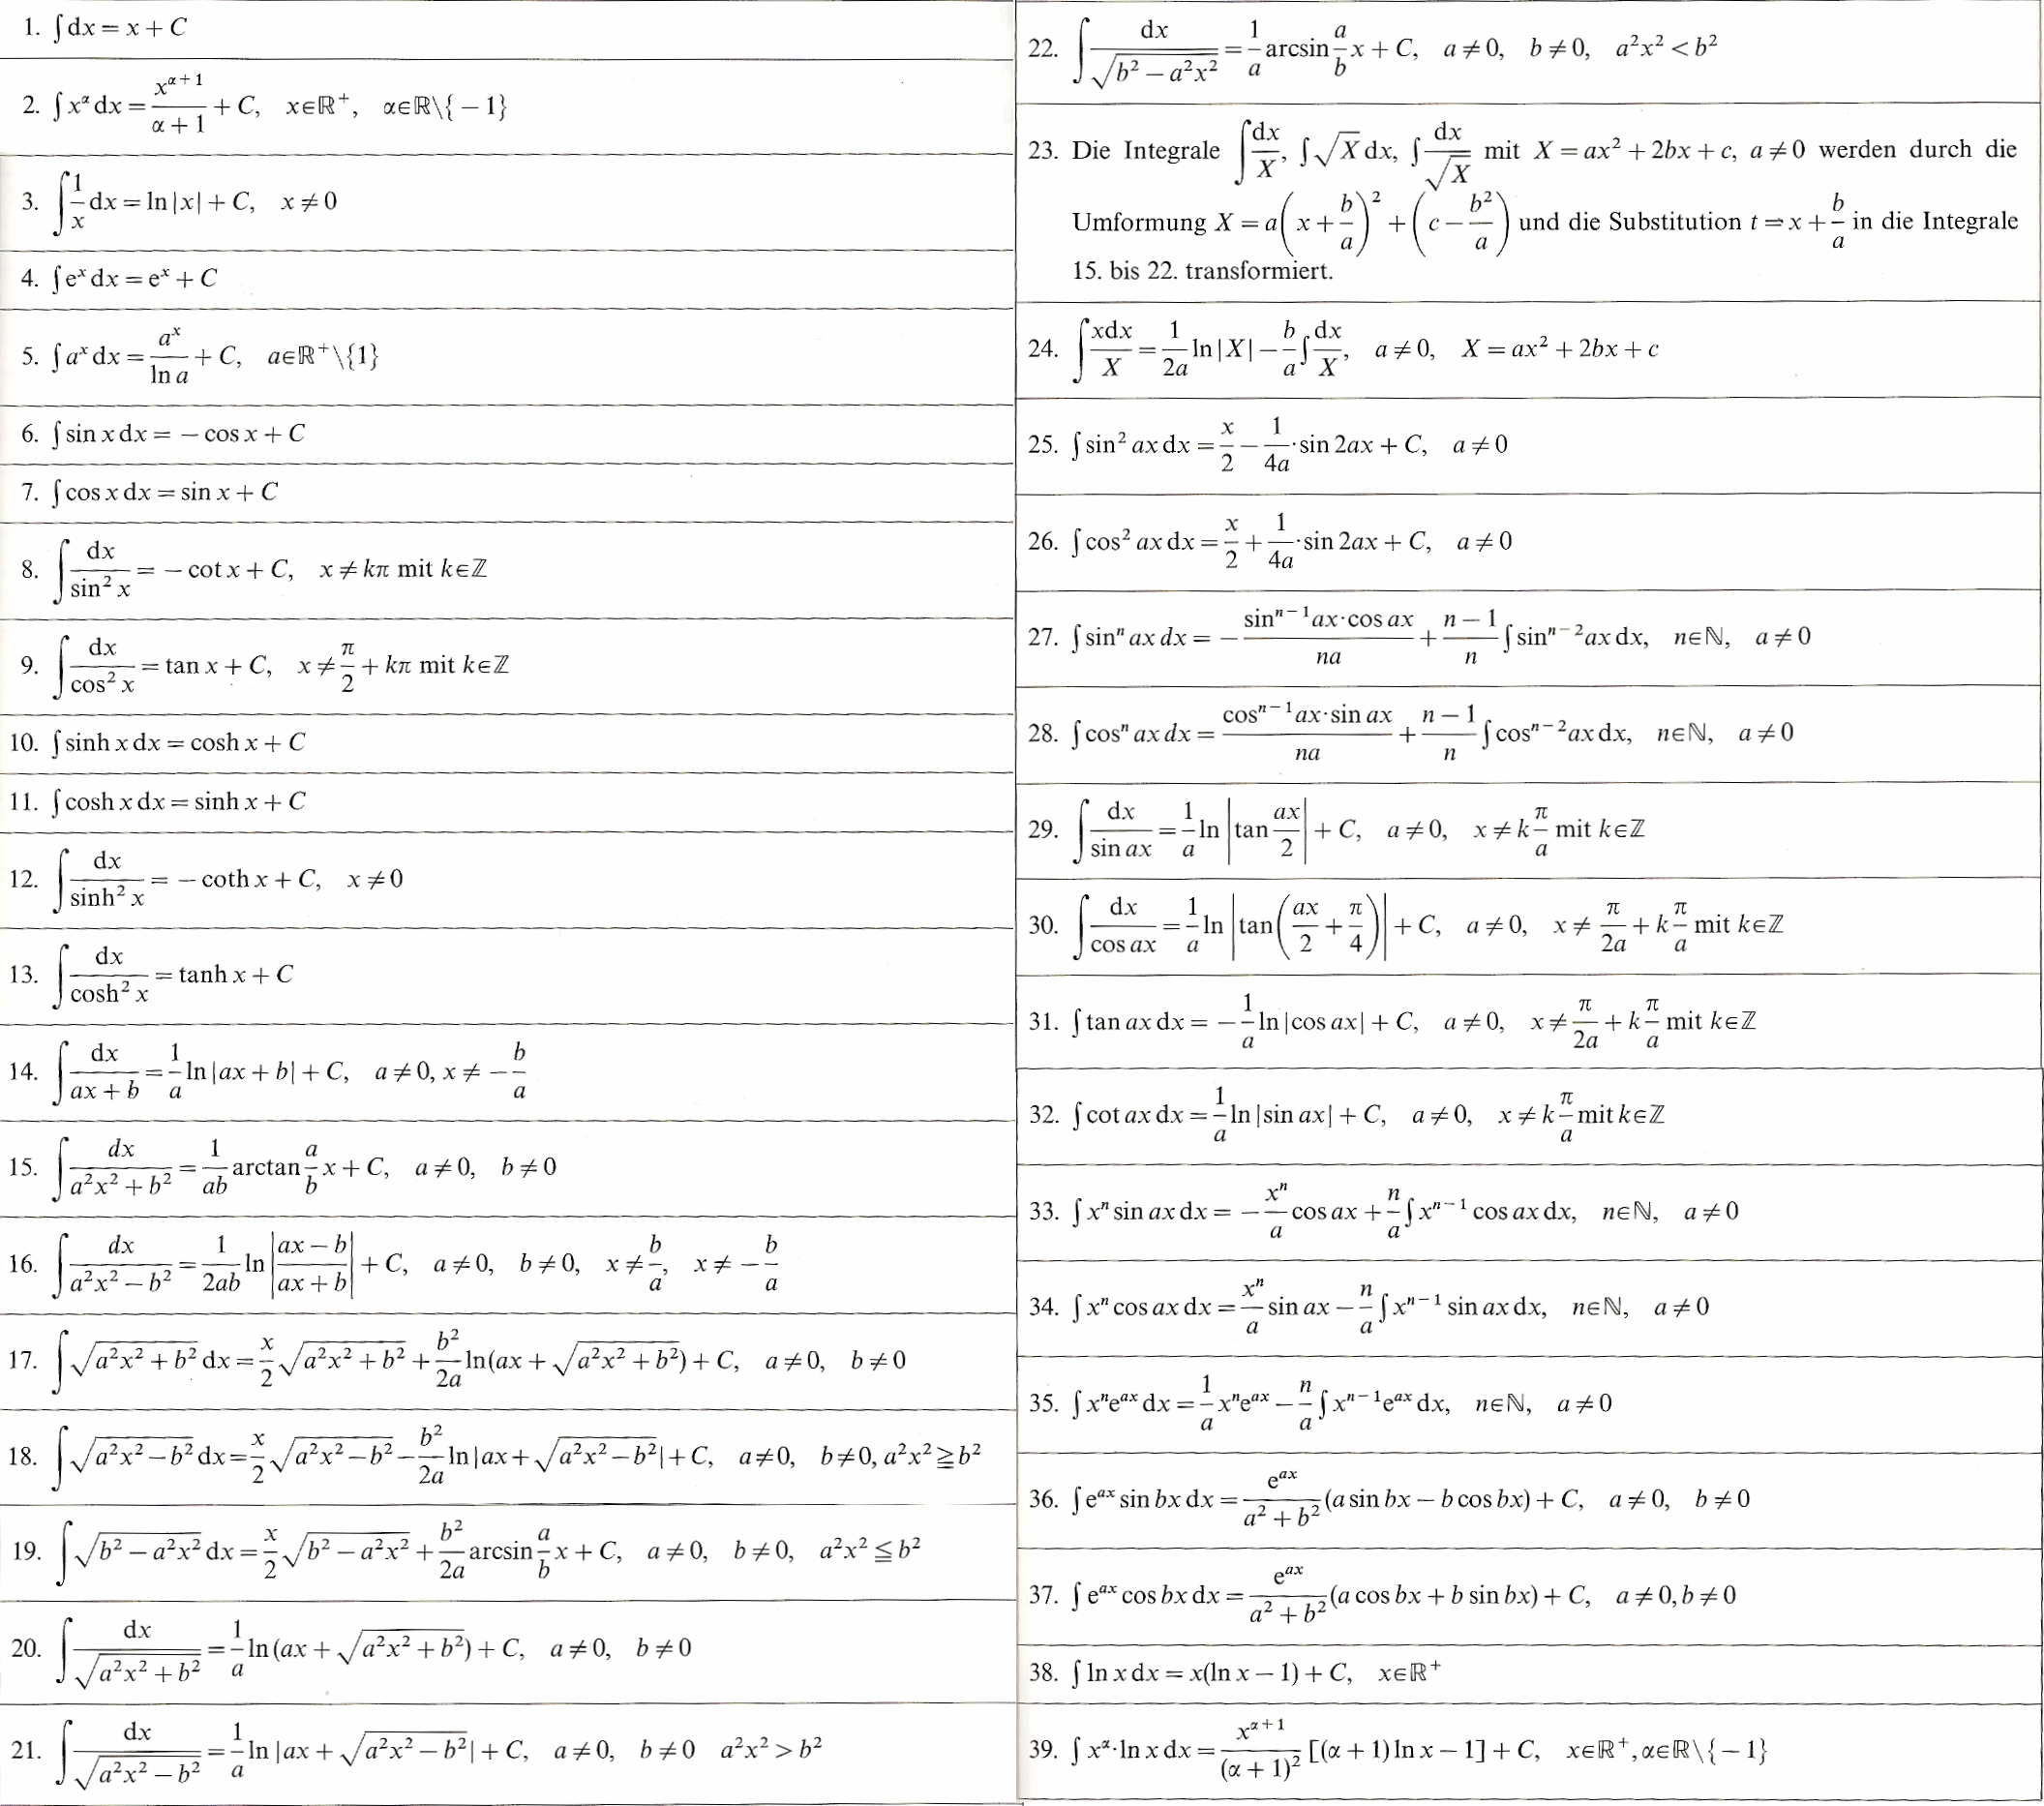
\includegraphics[width=16.1cm]{./bilder/integrale.png} 



\subsection{Uneigentliche Integrale\formelbuch{518}}
	Uneigentliches Integral heisst, dass entweder eine \textbf{unbeschränkte
	Funktion} integriert wird, oder eine Funktion über einen \textbf{unbeschränkten Integrationsberech} 
	integriert wird.$\\$
	\begin{minipage}{100mm}
    
	Für unbeschränkte Funktionen:$\\$
	$I =\int\limits _{a}^{c}f(x)dx=
	\lim\limits_{t\uparrow b}\int\limits_{a}^{t}f(x)dx+\lim\limits_{t\downarrow b}\int\limits_{t}^{c}f(x)dx\\
	\\$ Für die unbeschränkte Integration:$\\$
	$I =\int\limits _{a} ^{\infty} f(x)dx= \lim \limits_{t\to \infty}\int \limits
	_{a} ^{t}f(x)dx;\\$
	$I =\int\limits ^{a} _{-\infty} f(x)dx= \lim \limits_{t\to -\infty}\int
	\limits _{t} ^{a}f(x)dx; \\$
	$I =\int\limits _{-\infty} ^{\infty} f(x)dx = \lim \limits_{t_1\to -\infty} \lim
	\limits
	_{t_2 \to  \infty}\int \limits _{t_1} ^{a}f(x)dx + \int\limits_{a}^{t_2}f(x)dx\\$
	Beispiel: $\int\limits_{1}^{\infty}\frac{1}{x^2}dx=\lim\limits_{t\to \infty}\int\limits_{1}^{t}\frac{1}{x^2}dx=\lim\limits_{t\to \infty}-\frac{1}{t}+\frac{1}{1}=1$
    \end{minipage}
	\begin{minipage}{100mm}
    	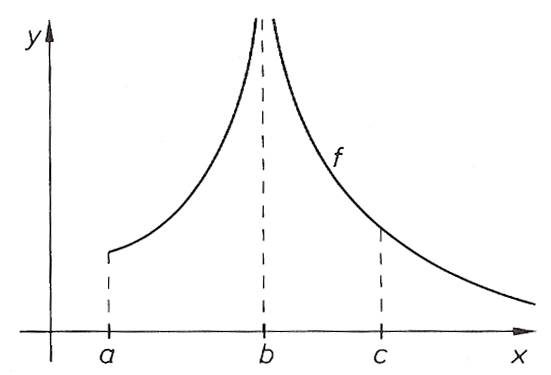
\includegraphics[width=3cm]{./bilder/unbeschraenkteFunktion.png} $\\$
    	unbeschränkte Funktion
    \end{minipage}

\subsubsection{Prinzip der Restfläche}
	Wenn $\lim\limits_{t \rightarrow \infty} \int\limits^{\infty}_{t} f(x) dx = 0$, dann konvergiert
	$\int\limits_a^{\infty} f(x) dx$ und umgekehrt.

\subsubsection{Majorantenprinzip}
	Um nachzuweisen, ob eine Funktion $|f(x)| \geq 0$ absolut konvergiert, wird eine zweite
	Funktion $g(x) \geq |f(x)|$ (Majorante) gesucht. Konvergiert $\int\limits_a^{\infty} g(x) dx$,
	dann konvergiert auch $\int\limits_a^{\infty} |f(x)| dx$ und somit konvergiert auch $\int\limits_a^{\infty} f(x) dx$. $\qquad x \in [a, \infty[$

\subsubsection{Minorantenprinzip}
	Um nachzuweisen, ob eine Funktion $f(x)$ divergiert, wird eine zweite
	Funktion $0 \leq g(x) \leq f(x)$ (Minorante) gesucht. Divergiert
	$\int\limits_a^{\infty} g(x) dx$,
	dann divergiert auch $\int\limits_a^{\infty} f(x) dx$. $\qquad x \in [a, \infty[$
	

%%%%%%%%%%%%%%%%%%%%%%%%%%%%%%%%%%%%%%%%%%%%%%%%%%%%%%%%%%%%%%%%%%%%%%%%%%%%%%%%%%%%%%%%%%%%%%%%
%%%%%%%%%%%%%%%%%%%%%%%%%%%%%%%%%%%%%%%%%%%%%%%%%%%%%%%%%%%%%%%%%%%%%%%%%%%%%%%%%%%%%%%%%%%%%%%%
%\newpage
\section{Anwendung der Differential- und Integralrechnung}

\subsection{Beschreibungungsvarianten}
	\begin{minipage}[t]{3.5cm}
		Funktion (explizit) \\
		$ y = f(x)$ \\
        \tiny{(Bronstein S.49, 147)}
	\end{minipage}
	\begin{minipage}[t]{6cm} 		
		Koordinatengleichung (implizit) \\
		$ F(x,y) = 0 $ \\
        \tiny{(Bronstein S.49)}
	\end{minipage}
	\begin{minipage}[t]{5.5cm} 		
		Parameterform(Cartesisch) \\
		$ \left( \begin{array} {l} x(t) \\ y(t) \end{array} \right) =
          \left( \begin{array} {l} \Psi(t) \\ \varphi(t) \end{array} \right)$\\
        \tiny{(Bronstein S.49)}
	\end{minipage} 
	\begin{minipage}[t]{3cm}
    	Polarform x\\
    	$ r=f(\varphi) $ \\
    \end{minipage}\\


	$\rightarrow$ Ordnung immer ohne $\sqrt{\text{ }}$ \\

\subsection{Umrechnen diverser Systeme \formelbuch{49}}
\begin{tabular}{| l l | l|}
\hline Parameter 
	& $\Rightarrow$ explizit
	%& $x = f(t) \; \; y = g(t)$
	& $ t = f(x);\; y = g(f(x))$\\
\hline Explizit
	& $\Rightarrow$ Parameter
	%& $y = f(x)$
	& $ \left( \begin{array} {l} x(t) \\ y(t) \end{array} \right) =
          \left( \begin{array} {l} t \\ g(t) \end{array}
          \right)$ \\
\hline Ex- bzw. implizit 
	& $\Rightarrow$ Polar
	%& $y = f_1(x)$ bzw. $f_2(x,y) = C$
	&  Ersetze $x = r \cos(\varphi)$ ; $y = r \sin(\varphi)$ ; $x^2+y^2 = r^2$\\ 
\hline Polar 
	& $\Rightarrow$ implizit
	%& $r = f(\varphi)$
	& Ersetze $r \sin(\varphi) = y$; $r \cos(\varphi)=x$; $r=\sqrt{x^2 + y^2}$\\ 
\hline Polar
	& $\Rightarrow$ Parameterform
	%& $r = f(\varphi)$
	& $\left( \begin{array} {l} x(\varphi) \\ y(\varphi) \end{array} \right) =
          \left( \begin{array} {l} r(\varphi) \cos(\varphi) \\ r(\varphi) \sin(\varphi) \end{array}
          \right)$ \\
\hline Einzelner Punkt  
	& $\Rightarrow$ Polar
	%& $(x,\; y)$
	& $r = \sqrt{x^2 + y^2};\;
	\varphi = \begin{cases}\arctan(\frac{y}{x}) + \pi 	&x < 0\\
             \arctan(\frac{y}{x}) 	& x > 0\\
             \frac{\pi}{2}			& x = 0;\; y > 0\\
             -\frac{\pi}{2}			& x = 0;\; y < 0\\
             \text{unbestimmt}		& x = y = 0\end{cases}$\\
\hline
\end{tabular}


\subsection{Kurvenarten\formelbuch{203ff}}
$ \left.\begin{matrix}
	\text{bei `+`, Kurve auf linke Seite geöffnet}\\ 
	\text{bei `-`, Kurve auf rechte Seite geöffnet}

\end{matrix}\right\rbrace $ 
bei Polarform

\begin{tabular}{llll}
\parbox{2.7cm}{
\textbf{ } \\
Implizit:\\
Bemerkung:\\
Polarform:\\
Parameterform:\\
$p, \epsilon$:
}

\parbox{6cm}{
\textbf{Kreis\formelbuch{203}}\\
$(x-x_0)^2 + (y - y_0)^2 = r^2$\\
Mittelpunkt $(x_0, y_0)$; Radius $r$\\
$r = \frac{p}{1 + \epsilon \cos(\varphi)}; \epsilon = 0$\\
$x=x_0 + R\cos(t), y=y_0 + R\sin(t) $ \\
$ p = \frac{b^2}{a}$
} 

\parbox{8cm}{
\textbf{Ellipse\formelbuch{204}}\\
$(\frac{x-x_0}{a})^2 + (\frac{y-y_0}{b})^2 = 1$\\
Mittelpunkt $(x_0, y_0)$; Halbachsen $a$, $b$\\
$r = \frac{p}{1 + \epsilon \cos(\varphi)}; 0 < \epsilon < 1 \qquad$ (rechter Brennpunkt)\\
$x = a\cos(t), y = b\sin(t) \qquad$ um $P(0,0)$ \\
$\epsilon = \frac{c}{a}$
}\\ \\


\parbox{2.7cm}{
\textbf {}\\
Implizit:\\
Bemerkung:\\
Polarform:\\
Parameterform:
}

\parbox{6cm}{
\textbf{Hyperbel\formelbuch{206}}\\ 
$(\frac{x}{a})^2 - (\frac{y}{b})^2 = 1; -(\frac{x}{a})^2 + (\frac{y}{b})^2 =1$\\ 
Achsenkreuz in $P(0,0)$\\
$r = \frac{p}{1 - \epsilon \cos(\varphi)}; \epsilon > 1_{(rechter Hyperbelast)}$\\
$r = \frac{p}{1 + \epsilon \cos(\varphi)}_{(linker Hyperbelast)}$ \\
$x= a \cosh(t), y = b \sinh(t) $ 

}

\parbox{8cm}{
\textbf{Parabel\formelbuch{209}}\\
$y^2 = 2p(x-x_0)$\\
Parabeln mit Scheitelpunkt auf der vertikaler Achse\\
$r = \frac{p}{1 - \epsilon \cos(\varphi)}; \epsilon = 1$\\
$x= \frac{t^2}{2p}, y = t$\\
$p=$Halbparameter (2$\cdot$Abstand Scheitel-Brennpunkt)
}\\ \\

\parbox{2.7cm}{
\textbf{} \\
Polarform:
}

\parbox{5cm}{
\textbf{Kardioide/Herzk. \formelbuch{99}} \\
$r = a(1+\cos(\varphi))$
}

\parbox{5cm}{
\textbf{Lemniskate ``$\infty$'' \formelbuch{101}} \\
$r = a\sqrt{2\cos(2\varphi)}$ 
}

\parbox{5cm}{
\textbf{Strophoide/harm. K. \formelbuch{96}} \\
$ r = -a \frac{\cos(2\varphi)}{\cos(\varphi)},(a>0) $ 
}

\end{tabular}

\subsection{Gleichungen, Mittelwerte\formelbuch{19ff, 509}}
\begin{tabular}{llll}
	\textbf{Tangentengleichung} &
	\textbf{Normalengleichung} &
	\textbf{Linearer Mittelwert} &
	\textbf{Quadratischer Mittelwert}\\
	$y-y_0=f'(x_0)(x-x_0)$ &
	$y-y_0=-\frac{1}{f'(x_0)}(x-x_0)$ &
	$\bar{f} = \frac{1}{b-a} \int\limits_{a}^{b} f(x)dx$ &
	$\bar{f} = \sqrt{\frac{1}{b-a} \int\limits_{a}^{b} f(x)^2dx}$ \\
	$\dot{x_0}(y-y_0) = \dot{y_0}(x-x_0)$ \\
\end{tabular}
	
\subsection{Tangenten- \& Normalenabschnitt, Subtangente \& Subnormale\formelbuch{251ff}}

\subsection{Abstandsformeln}
\begin{tabular}{p{7cm}p{5cm}p{6cm}l}
	\textbf{Hessesche Normalform\formelbuch{200f, 224}} &
	\textbf{Geradengleichung} &
	\textbf{Abstand zum Ursprung} \\
	$x\cdot \cos\varphi_0 +y\cdot \sin\varphi_0=r_0$ &
	$y - y_0 = m (x - x_0)$ &
	$\frac{|y_0 - m \cdot x_0|}{\sqrt{m^2 + 1}}$ \\
	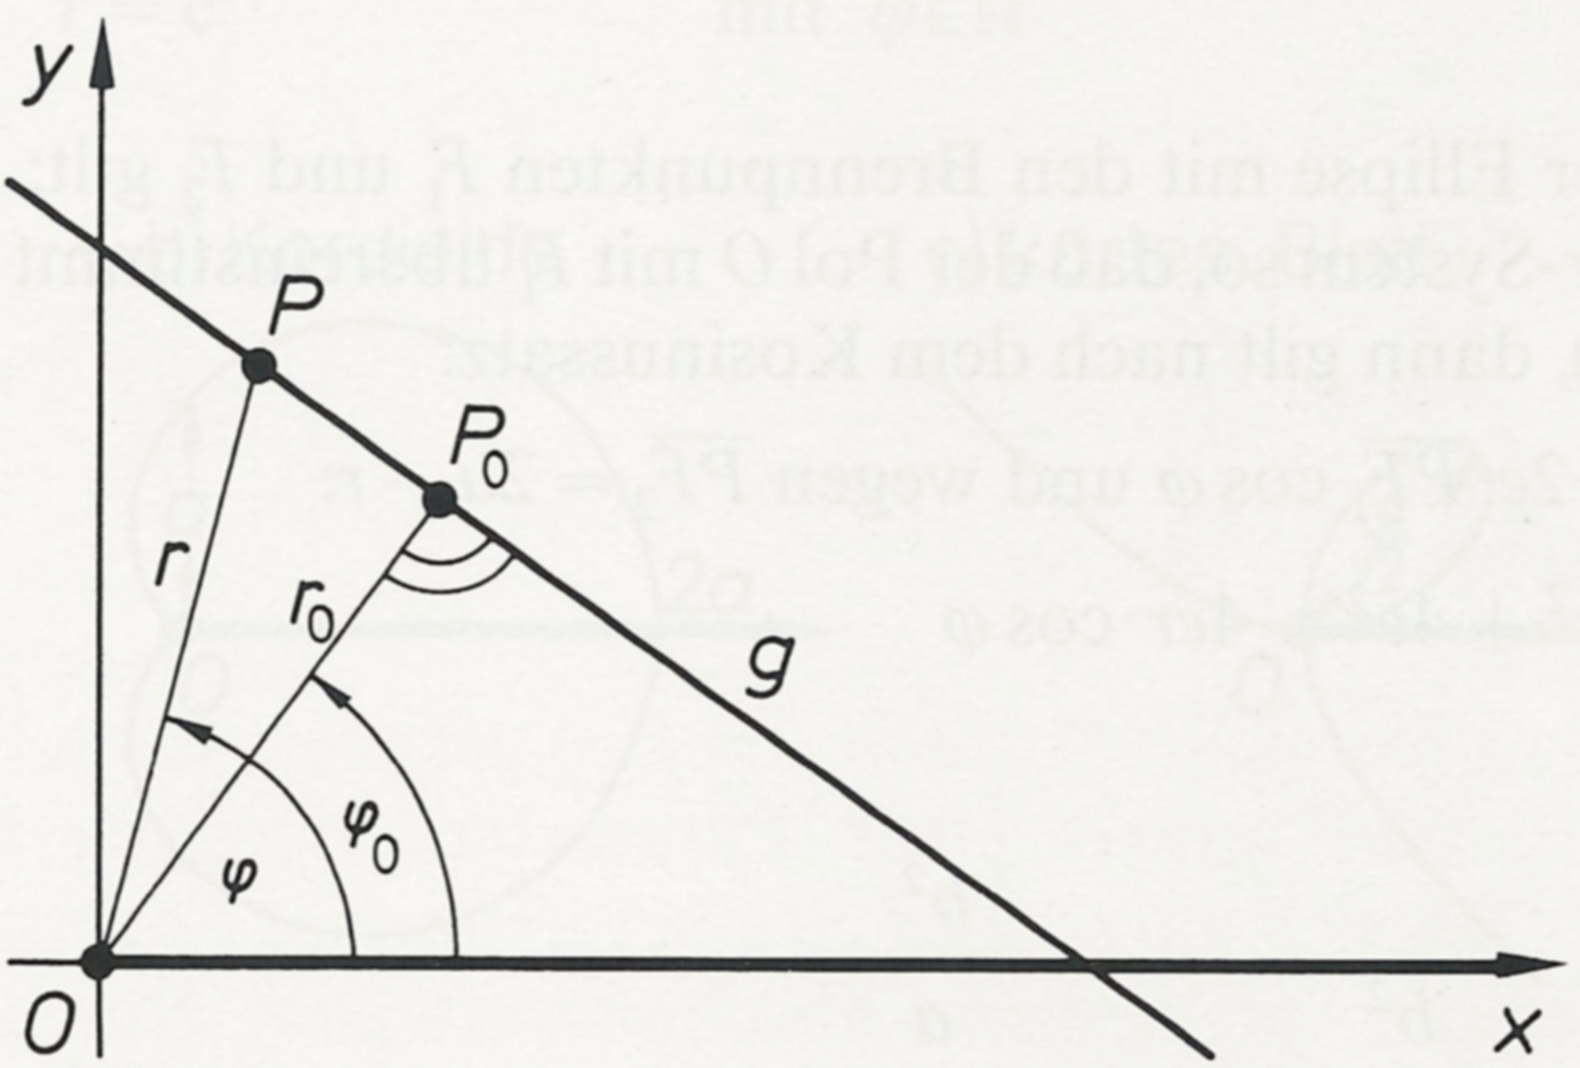
\includegraphics[width=6cm]{./bilder/hessenorm.png} \\
\end{tabular}


\subsection{Berührung in n-ter Ordnung}
Zwei explizit gegebene Kurven $y = f(x)$ und $y = g(x)$ berühren einander im
Punkt P $x_0, y_0$ von der Ordnung $n$, wenn die Funktionswerte und die ersten
$n$ Ableitungen existieren und übereinstimmen.\\
$f(x_0) = g(x_0);\; f'(x_0) = g'(x_0);\; f''(x_0) = g''(x_0);\;\ldots ;
\;f^{(n)}(x_0) = g^{(n)}(x_0)\; \qquad f^{(n+1)}(x_0) \neq g^{(n+1)}(x_0)$


\subsection{Scheitel \formelbuch{256}}

Scheitelpunte sind Extremalwerte der Krümmungs- bzw. Krümmungsradiusfunktion.
Falls bei $\kappa'(x)$ an der Stelle $x_0$ ein Vorzeichenwechsel besteht, existiert dort
eine Extremalstelle. 
$\qquad \kappa'(x) = 0; \kappa''(x) \neq 0$


\subsection{Wichtige Formeln\formelbuch{249ff}}
	\renewcommand{\arraystretch}{2}
	\begin{tabular}[c]{ | p{5.1cm} | p{5.4cm} | l | }
		\hline
		\textbf{Cartesisch} & \textbf{Parameter} & \textbf{Polar} \\
		\hline
		\multicolumn{3}{| l |}{\textbf{Anstieg einer Kurve, Ableitung, 2. Ableitung}} \\
    	\hline   
    	$y'=f'(x_o) \quad y'' = f''(x_0)$ & 
    	$y'=\frac{\dot{y}}{\dot{x}} \quad 
    	y'' = \frac{\dot{x} \ddot{y} - \dot{y}\ddot{x}}{\dot{x}^3}$ &
    	$y'=\frac{r'(\varphi) \sin(\varphi) + r(\varphi) \cdot
    	\cos(\varphi)}{r'(\varphi) \cos(\varphi)-r(\varphi) \cdot \sin(\varphi)}$
    	\\
		
		\hline
		\multicolumn{3}{| l |}{\textbf{Bogenlänge \formelbuch{514}}} \\
    	\hline
    	$s=\int\limits_a^b{\sqrt{1+(f'(x))^2}dx}$ & 
    	$|s|=\int\limits_{t_1}^{t_2}{\sqrt{\dot{x}^2(t)+\dot{y}^2(t)}dt}$ &
		$|s|=\int\limits_{\varphi_1}^{\varphi_2}{\sqrt{(r'(\varphi))^2+(r(\varphi))^2}d\varphi}$\\
		
		\hline		
		\multicolumn{3}{| l |}{\textbf{Krümmung ebener Kurven \formelbuch{253}}}\\
    	\hline
    	$\kappa=\frac{f''(x)}{(\sqrt{1+(f'(x))^2})^3}$ &
    	$\kappa=\frac{\dot{x}(t)\ddot{y}(t)-\dot{y}(t)\ddot{x}(t)}{(\sqrt{(\dot{x}(t))^2+(\dot{y}(t))^2})^3}$ &
		$\kappa=\frac{2(r'(\varphi))^2-r(\varphi)r''(\varphi)+(r(\varphi))^2}{(\sqrt{(r'(\varphi))^2+(r(\varphi))^2})^3}$\\   	
		
		\hline
		\multicolumn{3}{| l |}{Konvex (Linkskurve): $\kappa \geq 0 \qquad$ Streng
		konvex: $\kappa > 0 \qquad$ Wendepunkt: $\kappa = 0 \qquad$ Analog für konkav}\\
		
		\hline
		\multicolumn{3}{| l |}{\textbf{Krümmungskreisradius \formelbuch{253}} $\qquad r = |\frac{1}{\kappa}|$} \\
		\hline
		$r = \left|\frac{(\sqrt{1+(f'(x))^2})^3}{f''(x)} \right|$ &
		$r = \left|\frac{(\sqrt{(\dot{x}(t))^2+(\dot{y}(t))^2})^3}
		{\dot{x}(t)\ddot{y}(t)-\dot{y}(t)\ddot{x}(t)} \right|$ & 
		$r = \left|\frac{(\sqrt{(r'(\varphi))^2+(r(\varphi))^2})^3}
		{2(r'(\varphi))^2-r(\varphi)r''(\varphi)+(r(\varphi))^2} \right|$ \\
		
		\hline		
		\multicolumn{3}{| l |}{\textbf{Flächeninhalt \formelbuch{513}} um x-Achse /  für y-Achse: $f(y)$ von $y_0$ bis $y_1$ integrieren} \\
    	\hline
    	$A=\int\limits_a^b{f(x)}dx$  & 
    	$A=\frac{1}{2}\int\limits_{t_1}^{t_2}{[x(t)\dot{y}(t)-\dot{x}(t)y(t)]dt}$ &
		$A=\frac{1}{2}\int\limits_{\varphi_1}^{\varphi_2}{(r(\varphi))^2d\varphi}$\\  
    	
		\hline		
		\multicolumn{3}{| l |}{\textbf{Volumen \formelbuch{514}} um x-Achse 
		 / für y-Achse: $f(y)$ von $y_0$ bis $y_1$ integrieren
		 / Nur 1.Hälfte der Kurve integrieren!} \\
    	\hline
		$V=\pi\int\limits_a^b(f(x))^2dx$ & 
    	$V=\pi\left|\int\limits_{t_1}^{t_2}{(y(t))^2\dot{x}(t)dt}\right|$ &
		$V=\pi\left|\int\limits_{\varphi_1}^{\varphi_2}{r^2(\varphi)\sin^2\varphi[r'(\varphi)\cos(\varphi)-r(\varphi)\sin(\varphi)]d\varphi}\right|$\\  
    	
		\hline		
		\multicolumn{3}{| l |}{\textbf{Oberflächeninhalt \formelbuch{514}} um x-Achse 
		 / für y-Achse: $f(y)$ von $y_0$ bis $y_1$ integrieren
		 / Nur 1.Hälfte der Kurve integrieren!} \\
    	\hline
   		$O=2\pi\int\limits_a^b{|f(x)|\sqrt{1+(f'(x))^2}dx}$ & 
    	$O=2\pi\int\limits_{t_1}^{t_2}{|y(t)|\sqrt{\dot{x}^2(t)+(\dot{y}^2(t))}dt}$ &
		$O=2\pi\int\limits_{\varphi_1}^{\varphi_2}{|r(\varphi)\sin\varphi|\sqrt{(r'(\varphi))^2+(r(\varphi))^2}d\varphi}$\\  
    	\hline
		\multicolumn{3}{| l |}{Polar: \qquad $\sin \varphi =$ Drehung um Polgerade \qquad $\cos y =$ Drehung um y-Achse $(f = \frac{\pi}{2}) \qquad \rightarrow$ siehe Fläche} \\
	\hline
		\multicolumn{3}{| l |}{\textbf{Krümmungskreismittelpunkt}} \\
	\hline
		$x_c = x - \frac{\frac{dy}{dx}[1 + (\frac{dy}{dx})^2]}{\frac{d^2y}{dx^2}}$&
		$ x_c = x - \frac{\dot{y}(\dot{x}^2 + \dot{y}^2)}{\dot{x}\ddot{y} - \ddot{x}\dot{y}} $ &
		$x_c = r\cdot \cos\varphi - \frac{(r^2 + r'^2)(r\cdot \cos\varphi + r' \cdot \sin\varphi)}{r^2 + 2r'^2 - r\cdot r''}$\\

		$y_c = y + \frac{1+ (\frac{dy}{dx})^2}{\frac{d^2y}{dx^2}}$&
		$y_c = y + \frac{\dot{x}(\dot{x}^2 + \dot{y}^2)}{\dot{x}\ddot{y} - \ddot{x}\dot{y}} $ &
		$y_c = r\cdot \sin\varphi - \frac{(r^2 + r'^2)(r\cdot \sin\varphi - r' \cdot \cos\varphi)}{r^2 + 2r'^2 - r\cdot r''}$\\
	\hline
	\end{tabular}
	\renewcommand{\arraystretch}{1}
\subsection{Evolute}
Evolute = $\Sigma$ Krümmungskreiszentren\\
$\left(\begin{matrix} x_c \\ y_c \end{matrix}\right) = \left(\begin{matrix} x \\  y \end{matrix}\right) + \frac{1}{\kappa}\overrightarrow{n}$

\subsection{Orthogonaltrajektorien}
\begin{tabular}{ll}
\parbox{2.5cm}{
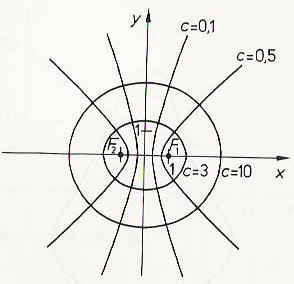
\includegraphics[height=2.5cm]{./bilder/orthoTrajekt.png}
}
& \parbox{16.5cm}{
Die orthogonalen Trajektorien schneiden alle Kurven der gegebenen Kurvenschar
$y=f(x,c)$ (c bestimmen) im rechten Winkel.
Die DGL $F(x,y,y')$ der Kurve bestimmen($y'$ ableiten, c einsetzen, wenn möglich für $f(x,c) = y$), anschliessend $y'$ durch
$-\frac{1}{y'}$ ersetzen.
$\Rightarrow$ ergibt die DGL der orthogonalen Trajektorien.\\
Die Kreise sind Orthogonaltrajektorien der Hyperbeln und umgekehrt.\\
$\frac{r'}{r} = f(\varphi , r) \qquad \underrightarrow{orthogonal}  \qquad \frac{r'}{r} = - \frac{1}{f(\varphi , r)}$
}
\end{tabular}

%%%%%%%%%%%%%%%%%%%%%%%%%%%%%%%%%%%%%%%%%%%%%%%%%%%%%%%%%%%%%%%%%%%%%%%%%%%%%%%%%%%%%%%%%%%%%%%%
%%%%%%%%%%%%%%%%%%%%%%%%%%%%%%%%%%%%%%%%%%%%%%%%%%%%%%%%%%%%%%%%%%%%%%%%%%%%%%%%%%%%%%%%%%%%%%%%
%newpage
\section{Reihen\formelbuch{469, 1073}}

\subsection{Zahlenreihen\formelbuch{470}}
$ s_n = \sum\limits_{k=1}^{n} a_k \qquad $ ist eine (unendliche) Reihe. Sie ist die Folge von Partialsummen einer bestehenden Folge $a_n$.

\subsubsection{Konvergenz, Divergenz\formelbuch{471}}
Konvergiert die Reihe $< s_n >$ gegen die Summe $ s = \sum\limits_{k=1}^{\infty} a_k $ so ist sie konvergent. 
Existiert der GW nicht, so ist sie divergent.

\subsubsection{Konvergenzkriterien\formelbuch{462}}

\paragraph{Cauchy-Kriterium} 
Wenn zu jedem $\varepsilon > 0$ ein Index $n_0$ existiert, so dass für alle $m > n > n_0$ gilt: \\
$\left| \sum\limits_{k=n}^m a_k \right| < \varepsilon$, dann konvergiert die Reihe, ansonsten divergiert sie.

\paragraph{lim = 0}
Wenn die Reihe $ \sum\limits_{n=1}^{\infty} a_n $ konvergent ist, so ist $\lim\limits_{n \to \infty} a_n = 0$. \hspace{2cm} Aber NICHT UMGEKEHRT!

\paragraph{Divergenz}
Ist $<a_n>$ divergent oder ist $\lim\limits_{n \to \infty} a_n \neq 0$, so ist die Reihe $ \sum\limits_{n=1}^{\infty} a_n $ divergent.

\paragraph{Majorantenkriterium\formelbuch{478}}
Ist die Reihe $ \sum\limits_{n=1}^{\infty} c_n $ konvergent, so konvergiert auch die Reihe $ \sum\limits_{n=1}^{\infty} |a_n|$ und somit auch
$\sum\limits_{n=1}^{\infty} a_n$ für $|a_n| \leq c_n$ (absolut).
Dies gilt auch für $|a_n| \leq c_n$ erst ab einer Stelle $n_0 \in \mathbb{N}$.\\
$\sum\limits_{n=1}^{m}a_k \leq |\sum\limits_{n=1}^{m}a_k| \leq \sum\limits_{n=1}^{m}|a_k| \leq \sum\limits_{n=1}^{m}c_n$

\paragraph{Minorantenkriterium}
Ist die Reihe $ \sum\limits_{n=1}^{\infty} d_n $ gegen $+\infty$ divergent, so gilt dies auch für die Reihe $ \sum\limits_{n=1}^{\infty} a_n $ 
bei $a_n \geq d_n$. \\ Dies gilt auch für $a_n \geq d_n$ erst ab einer Stelle $n_0 \in \mathbb{N}$. \\

\begin{tabular}{| p{4.5cm} | p{13.5cm} |}
	\hline
		\textbf{Reziprokkriterium} & 
		$ s = \sum\limits_{n=1}^{\infty} \frac{1}{n^\alpha} $ ist konvergent für $\alpha > 1$ und divergent für $\alpha \leq 1$.\\
	\hline
\end{tabular}

\begin{tabular}{| p{4.5cm} | p{8.5cm} | p{4.5cm} |}
	\hline
		\textbf{Quotientenkriterium}\formelbuch{473} &
		$ \lim\limits_{n \to \infty} \left|\frac{a_{n+1}}{a_n}\right| = \alpha $ der Reihe $ \sum\limits_{n=1}^{\infty} a_n$ &
		$\alpha < 1$ (aboslut) konvergent \\
	\cline{1-2}
		\textbf{Wurzelkriterium}\formelbuch{473} &
		$\lim\limits_{n \to \infty} \sqrt[n]{\left|a_n\right|} = \alpha $ der Reihe $ \sum\limits_{n=1}^{\infty} a_n$ &
		$\alpha = 1$ keine Aussage! \\
		&& $\alpha > 1$ divergent\\
	\hline
\end{tabular}

\begin{tabular}{| p{4.5cm} | p{13.5cm} |}
	\hline
		\textbf{Integralkriterium}\formelbuch{474} &
		$\int\limits_{1}^{\infty}f(x)dx$ konvergent $\Leftrightarrow \sum\limits_{n=1}^{\infty}f(n)$ konvergent. \\
		
		&Gilt nur, wenn $f$ auf $ [1, \infty) $ definiert und monoton fallend ($f'(x) \leq 0$) ist. \\
		&Zudem muss $ f(x) \geq 0 $ für alle $x \in [1, \infty)$ sein. \\
	\hline

		\textbf{Leibniz-Kriterium}\formelbuch{475} &
		Die \textbf{alternierende} Reihe $ \sum\limits_{n=1}^{\infty} a_n $ ist konvergent, wenn die Folge $<\left|a_n\right|>$ eine monoton fallende Nullfolge ($\lim\limits_{n \to \infty}
		\left|a_n\right| = 0 $) ist. Monotonie mittels Verhältnis ($ \left|\frac{a_{n+1}}{a_n}\right|$), Differenz ($ |a_{n+1}| - |a_n| \leq |a_{n+1}| $) oder \textit{vollständiger Induktion} beweisen.\\ 
	\hline
\end{tabular}
	
\paragraph{Abschätzung Restglied einer alternierenden konvergenten Reihe\formelbuch{471}}
	\qquad $|R_n| = |s-s_n|\leq |a_{n+1}|$


\subsubsection{Bedingte und Absolute Konvergenz\formelbuch{474}}
Eine Reihe $\sum\limits_{n=1}^{\infty}a_n$ heisst \textbf{absolut konvergent}, wenn die
Reihe $\sum\limits_{n=1}^{\infty}|a_n|$ konvergent ist.\\

\begin{tabular}{ p{4.5cm}  p{13.5cm}}
	\textbf{Bedingt Konvergent:} &  Eine Reihe hat durch Umordnen einen anderen Grenzwert oder wird divergent (somit nicht absolut konvergent).\\
	\textbf{Unbedingt Konvergent:} &  Durch Umordnen ändert sich der Grenzwert nicht.\\
\end{tabular}


\subsubsection{Produkt von absolut konvergenten Reihen\formelbuch{475}} 
Gegeben sei: $\sum a_n=a$, \quad $\sum b_n=b, \quad \sum c_n = (\sum a_n) \cdot (\sum b_n) = c \quad $ so ist
$ \quad c_n=\sum a_kb_{n-k+1} \quad $ und $ \quad c = a \cdot b $

\subsubsection{Fehlerformel}
	\qquad $|s_n-s|\leq |a_{n+1}|$

\subsection{Potenzreihen\formelbuch{481}}

\paragraph{Definition\formelbuch{432}} 
Die Reihe $ \sum\limits_{n=0}^{\infty} a_n (x-x_0)^n $ heisst Potenzreihe mit Entwicklungspunkt $x_0$ und Koeffizienten $a_n$.

\begin{tabular}{lll}
\textbf{Geometrische Reihe\formelbuch{19}}
	& $a \cdot \sum\limits_{n=0}^{\infty} q^n = \frac{a}{1-q}$
	& $(|q| < 1) \qquad$ Beidseitiges $\int \quad\Rightarrow\quad a \cdot \sum\limits_{n=1}^{\infty} \frac{q^{n}}{n} = -a \cdot \ln{|1-q|} $ \\
\textbf{Binominalreihe\formelbuch{12}} 
	& $\sum\limits_{n=0}^\infty \binom{\alpha}{n} x^n = (1+x)^\alpha$
	& $x \in (-1,1)\qquad$ Binominalkoeff. $\binom{n}{k} = \frac{n!}{(n-k)!k!} $\\
\textbf{Taylor-Reihe\formelbuch{483}}
	& $ \sum\limits_{n=0}^{\infty} \frac{f^{(n)}(x_0)}{n!}\cdot(x-x_0)^n$
	& Taylor-Reihe von f bezüglich der Stelle $x_0$ \\
\textbf{E-Funktion}
	& \multicolumn{2}{l}{$e = \lim\limits_{n\to\infty} \left(1+\frac{1}{n}\right)^n = 
	\sum\limits_{k=0}^{\infty}{\frac{1}{k!}} = 1 + \frac{1}{1} + \frac{1}{1\cdot 2} +
	\frac{1}{1\cdot 2\cdot 3}  + \frac{1}{1\cdot 2\cdot 3\cdot4} + \cdots$} \\

	&$e^x = \sum\limits_{n=0}^{\infty}\frac{1}{n!} \cdot x^n$ &
	für $x_0 = 0$
\end{tabular}

\subsubsection{Konvergenz\formelbuch{481}}
Gegeben sei die Potenzreihe $ \sum\limits_{n=0}^{\infty} a_n x^n $ mit $ \lim\limits_{n \to \infty} \sqrt[n]{|a_n|} = a $ oder $\lim\limits_{n \to \infty} |\frac{a_{n+1}}{a_n}| = a$ \\
Für $ a=0 $ ist die Potenzreihe für alle $ x \in \mathbb{R} $ absolut konvergent. \\
Für $ a>0 $ ist die Potenzreihe für alle $x$ mit 
$	\left\{ 	
		\begin{array}{l} 
			|x| < \frac{1}{a} = r \Rightarrow \text{ absolut konvergent.} \\
			|x| > \frac{1}{a} = r \Rightarrow \text{ divergent.}
		\end{array} 
	\right. $ \\
Ist die Folge $<\sqrt[n]{|a_n|}>$ nicht beschränkt, so ist die Potenzreihe nur für $x=0$ konvergent.

\subsubsection{Abel's Theorem}
$ \sum\limits_{n=0}^{\infty}a_n \cdot r^n$ konvergent  $= \lim\limits_{x \uparrow r}f(x)$ (= Summe der Reihe) 


\subsubsection{Konvergenzradius\formelbuch{481}}
Jeder Potenzreihe kann ein Konvergenzradius $r$ zugeordnet werden. Wobei gilt $r = \frac{1}{a}$ mit $a = \lim\limits_{n \to \infty} \sqrt[n]{|a_n|} $. \\
Für $a = 0$ gilt $r = \infty$. Wenn a nicht exisitiert (Folge divergent) ist $r = 0$. \\
Berechnung mittels Quotientenkriterium: $ r = \lim\limits_{n \to \infty} \left| \frac{a_n}{a_{n+1}} \right| = \lim\limits_{n\to\infty} \frac{1}{\sqrt[n]{|a_n|}}$

\subsubsection{Differentiation}
Alle Potenzreihen mit einem $\rho > 0$ sind für alle $x \in (-\rho, \rho)$ beliebig oft (gliedweise) differenzierbar. \\
Der Potenzradius $\rho$ ist bei allen Ableitungen gleich demjenigen der Ursprungsfunktion. $\rho_{f} = \rho_{f^{(i)}}$.
$$ f(x) = \sum\limits_{n=0}^{\infty} a_n x^n  \qquad 
   f'(x) = \sum\limits_{n=1}^{\infty} n \cdot a_n x^{n-1 } \qquad 
   f''(x) = \sum\limits_{n=2}^{\infty} n(n-1) \cdot a_n x^{n-2} \qquad 
   f^{(i)}(x) = \sum\limits_{n=i}^{\infty} n(n-1)\cdot \ldots \cdot (n-i+1)\cdot a_n x^{n-i} $$ 
\textbf{Bemerkung:} Startwert ($n=0$) nur erhöhen, wenn bei $x^n, n$ negativ werden würde!

\newpage
\subsubsection{Integration}
\paragraph{Unbestimmtes Integral}
$\int \sum\limits_{n=0}^{\infty} a_n x^n dx = 
\sum\limits_{n=0}^{\infty} a_n \int x^n dx = 
\sum\limits_{n=0}^{\infty} \frac{a_n}{n+1}\cdot x^{n+1} \qquad \text{ für alle } x \in (-\rho, \rho).$
\paragraph{Bestimmtes Integral}
$\int\limits_0^x \sum\limits_{n=0}^{\infty} a_n t^n dt = 
\sum\limits_{n=0}^{\infty} \frac{a_n}{n+1}\cdot x^{n+1} \qquad \text{ für alle } x \in (-\rho, \rho).$

\subsection{einige Reihen}

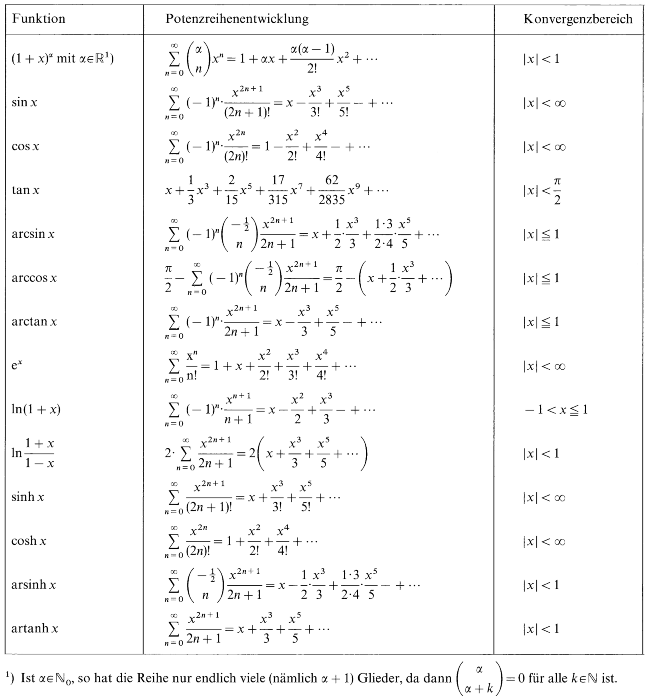
\includegraphics[height=17.0cm]{./bilder/reihen.png}

	Leibniz-Reihe: $ \sum\limits_{n=0}^{\infty} \frac{(-1)^n}{2^{n+1}} = 1-\frac{1}{3}+\frac{1}{5}-\frac{1}{7}+...+=\frac{\Pi}{4} $

	$\sum\limits_{n=1}^{\infty} \frac{1}{n} \rightarrow$ ist divergent \\
	$\sum\limits_{n=1}^{\infty} \frac{1}{n^2} \rightarrow$ absolut konvergent gegen 1 (beweisen mit Integralkriterium)

\subsection{Grenzwerte von Reihen}


\begin{tabular}{| l | l | l | l |}
	\hline
		$\lim\limits_{n\to\infty}(1+\frac{x}{n})^n = e^x$ &
		$\lim\limits_{n\to\infty}(\sqrt[n]{a}) = 1$ ($a > 0$ und const.) &
		$\lim\limits_{n\to\infty}(\sqrt[n]{n}) = 1$ &
		$\lim\limits_{n\to\infty}(\sqrt[n]{n^a}) = 1$ ($a$ const.)\\
	\hline
		$\lim\limits_{n\to\infty}(\sqrt[n]{|p(n)|}) = 1$ ($p(n) \neq 0$) &
		$\lim\limits_{n\to\infty}(\frac{K}{n!}) = 0$ ($K$ const.) &
		$\lim\limits_{n\to\infty}(\sqrt[n]{n!}) = +\infty$ &
		$\lim\limits_{n\to\infty}(\sqrt[n]{\frac{K^n}{n!}}) = 0$ ($K > 0$ und const.)\\
	\hline
		$\lim\limits_{n\to\infty}(\frac{n}{\sqrt[n]{n!}}) = e$ &&&\\
	\hline		
\end{tabular}

%%%%%%%%%%%%%%%%%%%%%%%%%%%%%%%%%%%%%%%%%%%%%%%%%%%%%%%%%%%%%%%%%%%%%%%%%%%%%%%%%%%%%%%%%%%%%%%%
%%%%%%%%%%%%%%%%%%%%%%%%%%%%%%%%%%%%%%%%%%%%%%%%%%%%%%%%%%%%%%%%%%%%%%%%%%%%%%%%%%%%%%%%%%%%%%%%

\section{Differentialgleichungen\formelbuch{552}}

\subsection{Lösen von Differentialgleichungen 1.Ordnung}

\subsubsection{Picard-Lindelöf}
Die Funktion $f(x, u, u_1, ..., u_{n-1})$ sei in einer Umgebung der Stelle $(x_0, y_0, y_1, ..., y_{n-1}) \in \mathbf{R^{n+1}}$ stetig und besitzt dort stetige partielle Ableitungen
nach $u, u_1, ..., u_{n-1}$ dann existiert in einer geeigneten Umgebung des Anfangspunktes $x_0$ genau eine Lösung des Anfangswertproblems\\
$y^{(n)} = f(x, y, y', ...,y^{(n-1)})$ mit $y(x_0) = y_0, y'(x_0) = y_1, ..., y^{(n-1)}(x_0) = y_{n-1}$ \\ \\
$\frac{\partial f}{\partial y}$ ... $\frac{\partial f}{\partial f^{(n-1)}}$ endlich beschränkt $\Rightarrow$ eindeutige Lösbarkeit



\subsubsection{Trennung von Variabeln / Separation \formelbuch{554}}
\begin{tabular}{p{4cm}p{1.5cm}p{10.5cm}}
\textbf{Form:} $y' = f(x) g(y)$ &
\textbf{Vorgehen:}              &
$\frac{y'}{g(y)} = f(x)$, nun ist die DGL beidseitig nach x integrierbar\\  &&
($dy = y'(x) dx$): $\int \frac{1}{g(y)} dy = \int f(x) dx$ 
\end{tabular}


\subsubsection{Lineartermsubstitution/separierte Lösung\formelbuch{554}}
\begin{tabular}{p{4cm}p{1.5cm}p{10.5cm}}
\textbf{Form:} $y'=f(ax+by+c)$   &
\textbf{Vorgehen:}               &
1. Substitution: $z=ax+by+c \qquad z'=a+by' =a+bf(z)$\\ &&

$\int\limits_{x_0}^{x}\frac{z'}{a+bf(z)}d\tilde{x} = \int 1 d\tilde{x} \Rightarrow \int\limits_{z_0}^{z}\frac{1}{a+bf(\tilde{z})}d\tilde{z} = \int\limits_{x_0}^{x}1 d\tilde{x} \qquad [d\tilde{z} = \underbrace{(a+by')}_{z'} d\tilde{x}]$
\end{tabular}

\subsubsection{Gleichgradigkeit\formelbuch{554}}
\begin{tabular}{p{4cm}p{1.5cm}p{15cm}}
\textbf{Form:} $y'=f(\frac{y}{x})$ &
\textbf{Vorgehen:}                &
1. Substitution: $z=\frac{y}{x} \qquad
z'=\frac{1}{x}(f(z)-z) \qquad
y'=f(z) \qquad
dz=y'(x)dx$ 
\end{tabular}

\subsubsection{Lineare Differentialgleichungen 1. Ordnung \formelbuch{555}}
\begin{tabular}{p{4.5cm}p{1.5cm}p{10.5cm}}
\textbf{Form:} $ y'+f(x)y = \underbrace{g(x)}_{\text{Störglied}} $ &
\textbf{Vorgehen:}                 &
$ y=e^{-\int f(x) dx}(k+\int g(x)e^{\int f(x)dx}dx) \qquad (k\in\mathbf{R})$
\end{tabular}


\subsection{Lineare Differentialgleichung 2. Ordnung mit konstanten Koeffizienten \formelbuch{573}}
\begin{tabular}{p{8cm}p{8cm}}
\textbf{Form:} $y''+a_1\cdot y'+a_0\cdot y=f(x)$  &
\textbf{Störglied:} $f(x)$\\
\textbf{Homogene Differentialgleichung:} $f(x)=0$ &
\textbf{Inhomogene Differentialgleichung:} $f(x)\neq 0$
\end{tabular}

\subsubsection{Allgemeine Lösung einer homogenen DGL:\quad\subsubadd{$\quad Y_H$}}
\textbf{Charakteristisches Polynom}
$\qquad\underline{\lambda^2+a_1\cdot\lambda+a_0=0}$ \hspace{1cm}von
$\qquad\underline{y''+a_1\cdot y'+a_0\cdot y=0}$ 
$\qquad(\lambda_{1,2} = -\frac{a_1}{2} \pm \frac{\sqrt{a_1^2 - 4a_0}}{2})$\\ \\

\begin{tabular}{p{2cm}p{5cm}p{6cm}p{4cm}}
$(D > 0)$ &
Falls $\lambda_1\neq \lambda_2$ und $\lambda_{1,2} \in R$: &
$Y_H=Ae^{\lambda_1x}+Be^{\lambda_2x}$ & 
$\rbrace$ starke Dämpfung\\

$(D = 0)$ &
Falls $\lambda_1=\lambda_2$ und $\lambda_{1,2} \in R$: &
$Y_H=e^{\lambda_1x}(A+B\cdot x)$ & 
$\rbrace$ aperiodischer Grenzfall\\

$(D < 0)$ &
Falls $\lambda_{1,2}=-\frac{a_1}{2}\pm j\alpha$: &
$Y_H=e^{-\frac{1}{2}a_1x}(Acos(\alpha x) +Bsin(\alpha x))$ &
$\rbrace$ schwache Dämpfung / Schwingfall \\
\end{tabular}

\begin{tabular}{p{2cm}p{5cm}p{2cm}p{4cm}}
	Eigenfrequenz: & $\omega = \alpha = \frac{\sqrt{|a_1^2 - 4a_0|}}{2}$ &
	Dämpfung: &  $|\delta| = |\lambda|$\\
\end{tabular}

\subsubsection{Allgemeine Lösung einer inhomogenen DGL:\quad\subsubadd{$y=Y_H+y_P$}}

\subsubsection{Grundlöseverfahren einer inhomogenen DGL:\quad\subsubadd{$\quad y_P$}}
Homogene DGL: $g(x) = Y_H$ mit den Anfangsbedingungen $g(x_0) = 0; g'(x_0) = 1$. Wenn möglich $x_0 = 0$.\\
$$y_P(x)=\int\limits_{x_o}^{x} g(x+x_0-t)\cdot f(t)dt$$	

\subsubsection{Vorgehen bei einer inh. DGL mit Störgliedtabelle: }
	Alle Schritte werden anhand diesem Beispiel erklärt: $\textcolor{red}{y'' + 3y' + 2y = 3e^{-2x}}$
	\begin{compactenum}
		\item 	$Y_H$ mit $\lambda_1$ und $\lambda_2$ berechnen \\
				\textcolor{red}{$y'' + 3y' + 2y = 0 \Rightarrow \lambda^2 + 3\lambda + 2 = 0 \Rightarrow \lambda_1 = -1$ und $\lambda_2 = -2 \Rightarrow Y_H = Ae^{-x} + Be^{-2x} \Rightarrow Y_{H1} = Ae^{-x}$ und $ Y_{H2} = Be^{-2c}$}
		\item 	Anhand der Störglied Tabelle $y_p$ bestimmen \\
				$\textcolor{red}{y_p = Ae^{-2x}}$
		\item 	Testen ob $y_p(x) = Y_{H1}$ oder $y_p(x) = Y_{H2}$ ist. 
				Falls Bedingung(en) zutreffen: $y_p(x)= y_p(x) * x^{\text{Anzahl zutreffende Bedingungen}}$ \\
				\textcolor{red}{$ y_p(x) = Y_{H2} \Rightarrow y_p(x) = Ae^{-2x}x $}
		\item 	$y_p$ ableiten und in die DGL einsetzen \\
				\textcolor{red}{$y_p'=(-2Ax + A)e^{-2x}$ und $y_p''=(4Ax - 4A)e^{-2x} \Rightarrow (4Ax - 4A)e^{-2x} + 3(-2Ax + A)e^{-2x} + 2Axe^{-2x} = 3e^{-2x}$}
		\item Gleichung kürzen und nach x-Potenzen ordnen \\
				\textcolor{red}{$(4A - 6A + 2A)xe^{-2x} + (3A - 4A)e^{-2x}=3e^{-2x}$}
		\item 	Koeffizienten bestimmen: \\				
				\begin{tabular}{ll}
					\textcolor{red}{$(3A - 4A) = 3$} & \textcolor{red}{$(3A - 4A)$} kommt 3 mal in $g(x)$ vor \\
					\textcolor{red}{$(4A - 6A + 2A) = 0$} & \textcolor{red}{$(4A - 6A + 2A)$} kommt 0 mal in $g(x)$ vor \\
				\end{tabular} \\
				$\textcolor{red}{A = -3}$
		\item 	Koeffizienten in $y_p$ einsetzen
				$\textcolor{red}{y_p = -3e^{-2x}}$
		\item 	Wenn das Störglied $f(x)$ aus mehreren Teilen besteht (z.B. $x^2e^x + x$), Störglied auseinander nehmen und in zwei Teile $x^2e^x$ und $x$ unterteilen und Schritt 3 - 6 wiederholen
		\item 	$y = Y_H + y_{p1} + y_{p2} + \dots$
	\end{compactenum}
	
\paragraph{Störgliedtabelle}
	\begin{tabular}{|p{8cm}|p{10cm}|}
		\hline 	
			Störglied $g(x)$ & Ansatz $y_p$ \\
		\hline
			$k$ (Konstante) & $A$ \\
		\hline
			$x^n$ & \multirow{2}{*}{$A_n*x^n + \dots + A_1*x + A_0$} \\
			$p_n(x) = b_n*x^n + \dots + b_1*x + b_0$ & \\
		\hline
			$k*e^{m*x}$ & $A*e^{m*x}$ \\
		\hline	
			$k*cos(b*x)$ & \multirow{3}{*}{$A*cos(b*x) + B*sin(b*x)$} \\
			$k*sin(b*x)$ & \\
			$k_1*cos(b*x) + k_2*sin(b*x)$ & \\
		\hline
			$k*e^{m*x}*cos(b*x)$ & \multirow{3}{*}{$e^{m*x}*(A*cos(b*x) + B*sin(b*x))$} \\
			$k*e^{m*x}*sin(b*x)$ & \\
			$e^{m*x}*(k_1*cos(b*x) + k_2*sin(b*x)$ & \\
		\hline
			$k*cosh(b*x)$ & \multirow{3}{*}{$A*cosh(b*x) + B*sinh(b*x)$} \\
			$k*sinh(b*x)$ & \\
			$k_1*cosh(b*x) + k_2*sinh(b*x)$ & \\
		\hline
			$k*e^{m*x}*cosh(b*x)$ & \multirow{3}{*}{$e^{m*x}*(A*cohs(b*x) + B*sinh(b*x))$} \\
			$k*e^{m*x}*sinh(b*x)$ & \\
			$e^{m*x}*(k_1*cosh(b*x) + k_2*sinh(b*x)$ & \\
		\hline
			$k*x*e^{mx}$ & $(A*x+B)*e^{m*x}$ \\
		\hline
			$p_n(x)*e^{m*x}$ & $(A_n*x^n + \dots + A_1*x + A_0)*e^{mx}$ \\
		\hline
			$x*(k_1*cos(b*x) + k_2*sin(b*x))$ & $(A_1*x+B_1)*cos(b*x) + (A_2*x+B_2)*sin(b*x)$ \\
		\hline
			$x*e^{mx}*(k_1*cos(b*x) + k_2*sin(b*x))$ & $e^{mx}*((A_1*x+B_1)*cos(b*x) + (A_2*x+B_2)*sin(b*x))$ \\
		\hline
			$x*(k_1*cosh(b*x) + k_2*sinh(b*x))$ & $(A_1*x+B_1)*cosh(b*x) + (A_2*x+B_2)*sinh(b*x)$ \\
		\hline
			$x*e^{mx}*(k_1*cosh(b*x) + k_2*sinh(b*x))$ & $e^{mx}*((A_1*x+B_1)*cosh(b*x) + (A_2*x+B_2)*sinh(b*x))$ \\
		\hline
	\end{tabular}
	\newpage

%%%%%%%%%%%%%%%%%%%%%%%%%%%%%%%%%%%%%%%%%%%%%%%%%%%%%%%%%%%%%%%%%%%%%%%%%%%%%%%%%%%%%%%%%%%%%%%%
%%%%%%%%%%%%%%%%%%%%%%%%%%%%%%%%%%%%%%%%%%%%%%%%%%%%%%%%%%%%%%%%%%%%%%%%%%%%%%%%%%%%%%%%%%%%%%%%

%\newpage
\subsubsection{Superpositionsprinzip}
$f(x)=c_1f_1(x)+c_2f_2(x)$\\
\begin{tabular}{p{8cm}p{8cm}}
$y_1$ ist spezielle Lösung der DGL &
$y_1''+a_1\cdot y_1'+a_0\cdot y_1=c_1f_1(x)$ \\
$y_2$ ist spezielle Lösung der DGL &
$y_2''+a_1\cdot y_2'+a_0\cdot y_2=c_2f_2(x)$ \\
dann ist:                          &
$y_P=c_1y_1+c_2y_2$\\
\end{tabular}

\subsection{Lineare Differentialgleichung n. Ordnung mit konstanten Koeffizienten \formelbuch{554}}
	\begin{tabular}{p{1.5cm}p{8cm}}
		\textbf{Form:} &
		$\sum\limits_{k=0}^na_ky^{(k)}= y^{(n)}+a_{n-1}\cdot y^{(n-1)}+\ldots +a_0\cdot y=f(x)$\\
	\end{tabular}

\subsubsection{n-verschiedene Homogene Lösungen}
	\begin{tabular}{lll}
		Fall a: r reelle Lösungen $\lambda_1$: 
			& $y_1=e^{\lambda_1x}$, $y_2=xe^{\lambda_1x}$, \ldots
			,$y_r=x^{r-1}e^{\lambda_1x}$ 
			& Starke Dämpfung / Kriechfall\\
		Fall b: $k$ komplexe Lösungen $\lambda_2=\alpha +j\beta$: 
			&$y_1=e^{\alpha x}\cos(\beta x)$, \ldots, $y_k=e^{\alpha x}x^{k-1}\cos(\beta
		x)$
			& Schwache Dämpfung /\\
			&$y_{k+1}=e^{\alpha x}\sin(\beta x)$, \ldots, $y_{2k}=e^{\alpha
		x}x^{k-1}\sin(\beta x)$
			& Schwingfall\\
	\end{tabular}
	$Y_H = Ay_1 + By_2 + Cy_3 + ... + Ny_n$

\subsubsection{Allgemeinste Lösung des partikulären Teils:}
	$$\underbrace{\sum_{k=0}^n a_k y^{(k)}}_{f(y,y',y'',\ldots)} = \underbrace{e^{\alpha x} (p_{m1}(x) \cos (\beta x) + q_{m2}(x) \sin (\beta x))}_{\text{Störglied}} \qquad \lambda \text{ aus Homogenlösung}$$
	Unterscheide die Lösungen des charakteristischen Polynoms ($\lambda$):\hspace{5.5cm}mit m = max(m1, m2)\\
	\begin{tabular}{p{8cm}p{8.5cm}}
		Fall a: $\alpha + j\beta \neq \lambda$, so ist &
		$y_P = e^{\alpha x}(r_m(x)\cos(\beta x) + s_m(x) \sin(\beta x))$\\
		Fall b: $\alpha + j\beta$  ist u-fache Lösung von $\lambda$, so ist &
		$y_P = e^{\alpha x} x^u (r_m(x) \cos(\beta x) + s_m(x) \sin(\beta x))$\\
		&
		u-fache Resonanz
	\end{tabular}

\subsubsection{Grundlöseverfahren}
	\begin{tabular}{p{12cm}p{5cm}}
		$\begin{pmatrix}
		g(x_0)=  & 0 & = & Ay_1(x_0)+By_2(x_0)+\ldots +Ny_n(x_0)\\
		g'(x_0)= & 0 & = & Ay_1'(x_0)+By_2'(x_0)+\ldots +Ny_n'(x_0)\\
		\vdots  & \vdots & \\                            
		g^{(n-1)}(x_0)= & 1 & = & Ay_1^{(n-1)}(x_0)+By_2^{(n-1)}(x_0)+\ldots
		+Ny_n^{(n-1)}(x_0)
		\end{pmatrix}$ &
		\begin{minipage}[t]{5cm}
			ergibt $c_1,\ldots ,c_n$ für\\
			$y_{P}(x)=\int\limits_{x_0}^x{g(x+x_0-t)f(t)dt}$
		\end{minipage}
	\end{tabular}

\subsubsection{Anfangswertproblem}
	$y(x_0) = y_0 \qquad y'(x_0) = y_1 \qquad y''(x_0) = y_2 \qquad \dots \qquad y^{(n-1)}(x_0) = y_{n-1}$


\subsection{Lineare Differentialgleichungssysteme erster Ordnung mit konstanten Koeffizienten}
	\begin{tabular}{p{8cm}p{8cm}}
		\textbf{Form:}& $	\begin{matrix} \dot{x}=ax+by+f(t) \\ \dot{y}=cx+dy+g(t) \end{matrix} = \left(\begin{matrix} \dot{x} \\ \dot{y} \end{matrix}\right) = 
					\left(\begin{matrix} a & b \\ c & d \end{matrix}\right) \left(\begin{matrix} x \\ y \end{matrix}\right) + \left(\begin{matrix} f(t) \\ g(t) \end{matrix}\right)$ \\
	
	
		\textbf{Die allgem. Lösung ergibt sich aus der DGL:}&
		$\underbrace{\ddot{x}-(a+d)\dot{x}+(ad-bc)x=\dot{f}(t)-df(t)+bg(t)}_{\text{normale DGL 2.Ordnung} \rightarrow \text{nach $x$ auflösen}}$\\
		& $y=\frac{1}{b}(\dot{x}-ax-f(t)))$\\
	
		\textbf{Anfangsbedinung:} &
		$x_0(t_0) = x_0, \dot{x}_0(t_0) = ax_0 + by_0 + f(t_0)$
	\end{tabular} \\ \\
	\textbf{Anordnung beachten!} Gesuchte Grösse immer zu oberst (in diesem Fall ist die gesuchte Grösse $x$)

\subsection{Faltung \formelbuch{802}}
	$f(x) = \int\limits_0^x f_1(x-t)f_2(t) dt \qquad$ Schreibweise $f = f_1 *  f_2$

\newpage
\section{Formeln + Theorie aus An1E}

%%%%%%%%%%%%%%%%%%%%%%%%%%%%%%%%%%%%%%%%%%%%%%%%%%%%%%%%%%%%%%%%%%%%%%%%%%%%%%%%%%%%%%%%%%%%%%%%
% Trigonometrie
%%%%%%%%%%%%%%%%%%%%%%%%%%%%%%%%%%%%%%%%%%%%%%%%%%%%%%%%%%%%%%%%%%%%%%%%%%%%%%%%%%%%%%%%%%%%%%%%	
\subsection{Trigonometrie}
	$\sin^2(b)+\cos^2(b)=1 \qquad \tan(b)=\frac{\sin(b)}{\cos(b)}$
	
\subsubsection{Funktionswerte für Winkelargumente}
	\renewcommand{\arraystretch}{1.5}
	\begin{minipage}{5cm}
		\begin{tabular}[c]{ |c|c||c|c|c| }
	    	\hline
			deg & rad & sin & cos & tan\\
			\hline
			0\symbol{23} & 0 & 0 & 1 & 0\\
			\hline
			30\symbol{23} & $\frac{\pi}{6}$ & $\frac{1}{2}$ & $\frac{\sqrt{3}}{2}$ &
			$\frac{\sqrt{3}}{3}$\\
			\hline
			45\symbol{23} & $\frac{\pi}{4}$ & $\frac{\sqrt{2}}{2}$ & $\frac{\sqrt{2}}{2}$
			& 1\\
			\hline
			60\symbol{23} & $\frac{\pi}{3}$ & $\frac{\sqrt{3}}{2}$ & $\frac{1}{2}$ &
			$\sqrt{3}$\\
			\hline			
		\end{tabular}			
	\end{minipage}
	\begin{minipage}{4.3cm}
		\begin{tabular}[c]{ |c|c||c|c|}
	    	\hline
			deg & rad & sin & cos\\
			\hline
			90\symbol{23} & $\frac{\pi}{2}$ & 1 & 0\\
			\hline	
			120\symbol{23} & $\frac{2\pi}{3}$ & $\frac{\sqrt{3}}{2}$ & $-\frac{1}{2}$ \\
			\hline
			135\symbol{23} & $\frac{3\pi}{4}$ & $\frac{\sqrt{2}}{2}$ & $-\frac{\sqrt{2}}{2}$\\
			\hline
			150\symbol{23} & $\frac{5\pi}{6}$ & $\frac{1}{2}$ & $-\frac{\sqrt{3}}{2}$\\
			\hline
		\end{tabular}			
	\end{minipage}
	\begin{minipage}{4.5cm}
		\begin{tabular}[c]{ |c|c||c|c| }
	    	\hline
			deg & rad & sin & cos\\
			\hline
			180\symbol{23} & $\pi$ & 0 & -1\\
			\hline	
			210\symbol{23} & $\frac{7\pi}{6}$ & $-\frac{1}{2}$ & $-\frac{\sqrt{3}}{2}$\\
			\hline
			225\symbol{23} & $\frac{5\pi}{4}$ & $-\frac{\sqrt{2}}{2}$ & $-\frac{\sqrt{2}}{2}$\\
			\hline
			240\symbol{23} & $\frac{4\pi}{3}$ & $-\frac{\sqrt{3}}{2}$ & $-\frac{1}{2}$\\
			\hline
		\end{tabular}			
	\end{minipage}
	\begin{minipage}{4.5cm}
		\begin{tabular}[c]{ |c|c||c|c| }
	    	\hline
			deg & rad & sin & cos\\
			\hline
			270\symbol{23} & $\frac{3\pi}{2}$ & -1 & 0\\
			\hline	
			300\symbol{23} & $\frac{5\pi}{3}$ & $-\frac{\sqrt{3}}{2}$ & $\frac{1}{2}$\\
			\hline
			315\symbol{23} & $\frac{7\pi}{4}$ & $-\frac{\sqrt{2}}{2}$ & $\frac{\sqrt{2}}{2}$\\
			\hline
			330\symbol{23} & $\frac{11\pi}{6}$ & $-\frac{1}{2}$ & $\frac{\sqrt{3}}{2}$\\
			\hline
		\end{tabular}			
	\end{minipage}
	\renewcommand{\arraystretch}{1}
	
\subsubsection{Periodizität}
	$\cos(a+k\cdot2\pi)=\cos(a) \qquad \sin(a+k\cdot2\pi)=\sin(a) \qquad
	(k \in \mathbb{Z})$
	
\subsubsection{Quadrantenbeziehungen}
	\begin{tabbing}
    	xxxxxxxxxxxxxxxxxxxxxxxxxxxxxxxxxx \= \kill
	 	$\sin(-a)=-\sin(a)$ \> $\cos(-a)=\cos(a)$\\
		$\sin(\pi - a)=\sin(a)$ \> $\cos(\pi - a)=-\cos(a)$\\
		$\sin(\pi + a)=-\sin(a)$ \> $\cos(\pi +a)=-\cos(a)$\\
		$\sin\left(\frac{\pi}{2}-a \right)=\sin\left(\frac{\pi}{2}+a \right)=\cos(a)$ \>
		$\cos\left(\frac{\pi}{2}-a \right)=-\cos\left(\frac{\pi}{2}+a \right)=\sin(a)$  
    \end{tabbing}

\subsubsection{Additionstheoreme}
		$\sin(a \pm b)=\sin(a) \cdot \cos(b) \pm \cos(a) \cdot \sin(b)$\\
		$\cos(a \pm b)=\cos(a) \cdot \cos(b) \mp \sin(a) \cdot \sin(b)$\\	
		$\tan(a \pm b)=\dfrac{\tan(a) \pm \tan(b)}{1 \mp \tan(a) \cdot \tan(b)}$

\subsubsection{Doppel- und Halbwinkel}	
		$\sin(2a)=2\sin(a)\cos(a)$\\
		$\cos(2a)=\cos^2(a)-\sin^2(a)=2\cos^2(a)-1=1-2\sin^2(a)$\\
		$\cos^2 \left(\frac{a}{2}\right)=\frac{1+\cos(a)}{2} \qquad
		\sin^2 \left(\dfrac{a}{2}\right)=\frac{1-\cos(a)}{2}$
		
\subsubsection{Produkte}
		$\sin(a)\sin(b)=\frac{1}{2}(\cos(a-b)-\cos(a+b))$\\
		$\cos(a)\cos(b)=\frac{1}{2}(\cos(a-b)+\cos(a+b))$\\
		$\sin(a)\cos(b)=\frac{1}{2}(\sin(a-b)+\sin(a+b))$
		
\subsubsection{Summe und Differenz}
		$\sin(a)+\sin(b)=2 \cdot \sin \left(\frac{a+b}{2}\right) \cdot
		\cos\left(\frac{a-b}{2}\right)$\\
		$\sin(a)-\sin(b)=2 \cdot \sin \left(\frac{a-b}{2}\right) \cdot
		\cos\left(\frac{a+b}{2}\right)$\\
		$\cos(a)+\cos(b)=2 \cdot \cos \left(\frac{a+b}{2}\right) \cdot
		\cos\left(\frac{a-b}{2}\right)$\\
		$\cos(a)-\cos(b)=-2 \cdot \sin \left(\frac{a+b}{2}\right) \cdot
		\cos\left(\frac{a-b}{2}\right)$\\
		$\tan(a) \pm \tan(b)=\dfrac{\sin(a \pm b)}{\cos(a)\cos(b)}$		
	
\end{document}
